\documentclass[10pt,a4paper,twocolumn]{report}

\usepackage[utf8]{inputenc}
\usepackage{amsmath}
\usepackage{amsfonts}
\usepackage{amssymb}
\usepackage[utf8]{inputenc}
\usepackage[pdftex]{graphicx}
\usepackage{newunicodechar}


\begin{document}

\title{Whereabouts Clock}
\author{Byeonggon Lee,Jaehyun Byeon,Sowon Park,Juhyeok Bae}
\maketitle



%\begin{table}[]
%\centering
%\caption{Role assignment}
%\begin{tabular}{ccc}
%	\multicolumn{1}{c|}{Roles} & \multicolumn{1}{c|}{Names} & Task description and etc. \\ \hline
%	\multicolumn{1}{c|}{User} & \multicolumn{1}{c|}{Sowon Park} &  supposing herself as an 
%	end-user of this software, listed both predictable inconveniences and desired properties.\\ %\hline
%	\multicolumn{1}{c|}{Customer} & \multicolumn{1}{c|}{Jaehyun Byeon} & Make concrete which %functions are necessary. When 
%	user purchase this software, customer analysis the benefits of this software.  \\ \hline
%	\multicolumn{1}{c|}{Software Developer} & \multicolumn{1}{c|}{Juhyeok Bae} & Plan how to %implement this %software, 
%	consider the algorithm and system within software \\ \hline
%	\multicolumn{1}{c|}{Developer Manager} & \multicolumn{1}{c|}{Byeonggon Lee} & design a general idea of this %software,	
%	managing our team. \\ \hline
%\end{tabular}
%\end{table} 


\textbf{abstract}- Overall, our real time location clock has two purposes. First, by informing families at home of each member’s location, they can be relieved. Second, by automatically showing information at clock, people can be aware of each other's location fast and conveniently than using a phone call or messenger. We provide this service with smart phone application and clock equipped with Raspberry pi. Application server compares initial user's setup data and their real time location using Own tracks application. If the data corresponds to the setup data stored at Database, Application Server sends request to change the hands of clock which indicate family member’s location. Our clock provides each locations of member and reduces concerns about safety. \\
\textbf Role Assignment \\

\begin{figure}[h]
		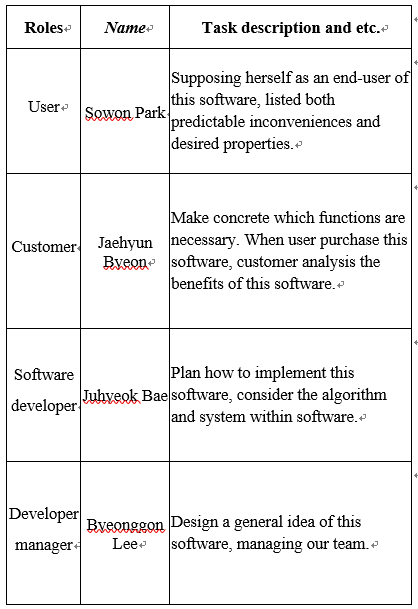
\includegraphics[width=0.5\textwidth]{Figure4.png}
		\caption{Catpion1}
		\label{fig1}
\end{figure} 

\section{Introduction}
	Modern society is composed of various social groups. From birth, we belong to a family and get to be part of a peer group as we grow up. The relationship between the group members has been more important since we usually have a strong sense of belonging to it. Among many social groups, a family would be the most crucial social group because we naturally belong to it from birth. 
     Members of a family share a strong bond which is connected emotionally. When children are young, there are usually a lot of opportunities to spend time with their parents. However, as children grow up to be adults and can take care of themselves, it becomes difficult to have enough face-to-face conversations for a family. Both sides often try to keep their sense of family’s closeness by phone calls or sending messages. Therefore, the most common question in a family would be asking where the other person is. This is because the most important thing for a family is consistently checking the safety of each other. 
     With this mind, our team has come up with an idea to provide a service that can let the family members know the location of each other easily. There are already many applications in the field that someone can track the exact location of family members. We decided to use that service as our basic idea and come up with something that can present the information in visual forms and sounds. The technology would be applied to the clock because it is easy for us to see in their everyday lives. Whereabouts clock will show the location of each family member instead of only showing the physical time as normal clock does. 
     Our location clock service consists of these things as stated below. The hands of the clock will represent the family members. The clock will use a hardware called the raspberry pi to get information from the application. The application will retrieve information data using the ‘Own tracks’ application. The information of the users will be stored in the database through the server where their location data would be checked in real-time. The specific fundamentals of this clock’s IOT function would be presented more clearly in the specification sector. 
     We would also like to further implement this technology to not only just family members but also to others in need. This clock service could be used in places such as hospitals, or facilities that should take care of young or old people. As the number of caretakers of such places are limited and they still need a lot of help, we would like to provide a service that would aid them with informing the location of the people through visual and sound methods using a form of a clock.
     

\section{Requirement}
	\subsection{Requirement for Clock}
		%\begin{enumerate}
		\subsubsection{0.2.1.1. Clock kit} 
		- An old beat up clock or old clock shell \\
		- 1 raspberry pi Micro-Computer \\
		- 3 Sail winch servos (special servos that can turn 360 degrees)\\
		- A middle device that connects between raspberry pi and 3 Sail winch servo \\
		- 3 Brass Tubes (one is 1/4 inch, another is 9/32 inch, the other is the          
		  smallest one) and 6 gear \\
		- For additional function, 1 display panel and 1 speaker \\
		
		\subsubsection{0.2.1.2. Network} 
		- To connect raspberry pi with Wi-Fi, we should connect Wi-Fi dongle with 
		  raspberry pi \\
		  
		\subsubsection{0.2.1.3. Receiving data} 
		- Connecting the Wi-Fi to receive the GPS data from the Application with clock \\
        - Connecting the Wi-Fi to receive the short message that user send\\

		\subsubsection{0.2.1.4. Handling input data} 
		- To judge where the clock hands should move to \\
		
		\subsubsection{0.2.1.5. Moving clock hands} 
		- Move clock hands in real time \\
		
		\subsubsection{0.2.1.6. Floating the message} 
		- Floating the short message that family sends shortly \\
		
		\subsubsection{0.2.1.7. Alarm} 
		- If the family location changes, clock alarms the user  \\
		
		\subsubsection{0.2.1.8. Informing the real time} 
		- Display panel on the bottom showing the real time \\
        - Ex) 2017.04.01 10 pm \\

	\subsection{Requirement for Application}
		\subsubsection{0.2.2.1. Install application}
		
		\subsubsection{0.2.2.2. Sign in and login}

		\subsubsection{0.2.2.3. Permitting to give users GPS data.}

		\subsubsection{0.2.2.4. Making the family group}
		- Set the family number \\
		- The main user invites other family member \\
		- Connecting with the clock \\

		\subsubsection{0.2.2.5. Setting the default location information ex) school – GPS data}

		\subsubsection{0.2.2.6. Comparing the real time GPS data with default location data}
		- Handling between the real time GPS data and default location information that setting \\
		
		\subsubsection{0.2.2.7. Transmit data that compare between the real time GPS data and default location data to clock}
		- If the status of one application is on, the application server sends a GPS data to clock \\
		
		\subsubsection{0.2.2.8. Sending user message and setting states}
		- User can send a short message to the clock screen. \\
		- When user click the button which represents location state like (Moving, Studying, Working, and Taking a rest or so 
		  on), application changes the clock screen display. \\
 
     \subsection{Requirement for User}
     	\subsubsection{0.2.3.1. Install Whereabouts clock}
     	- User is required to get the clock. \\
		- User puts a battery in the clock. \\
		
		\subsubsection{0.2.3.2. Set up family data with hands of clock.}
     	- User makes each hand of clock indicate family members. \\
		- User puts place to confirm family’s location instead of time in clock.\\
		
		\subsubsection{0.2.3.3. Join and sign in smartphone application}
     	- Family members are required to make an account with his/her email address or phone number and 		  password in the application.\\
		- User can sign in with the setting of email address or phone number and password that he/she 			  registered at the first time.\\
		
 		\subsubsection{0.2.3.4. Make a group in the smartphone application}
     	- One of family member should invite the others to group setting.\\
     	
     	\subsubsection{0.2.3.5. Connect the setting between members and hands of clock}
     	- Each member set the application to make watch point themselves. \\
     	
		\subsubsection{0.2.3.6. Register user’s clock}
     	- To connect clock with the application, user should register clock and network path. 			
     	Application considers where and how to send the input data.\\
     	
     	\subsubsection{0.2.3.7. Create user settings in Database}
     	- User should register the setup location which they want to represent in Database. If they 
     	want to set their home, they can store home address in the application and the server store as 
     	they received data in database.\\
 		- User also can resister other locations they want to confirm. For example, there could be 	
 		parent’s company locations, children’ school locations, children’s private educational 
 		institutes and so on.\\
 		
		\subsubsection{0.2.3.8. Register basic application settings}
     	- User should set the checking time(for 30 seconds of one minute ) when the application 		          retrieves user’s real time location.\\
     	- User should allow the application to take user’s GPS data.\\
     	
     	\subsubsection{0.2.3.9. Click the state button }
     	- When user want to represent their current conditions to other family’s members, he or she can 		  press the button which represents their present states. \\
     	
     	\subsubsection{0.2.3.10. Listen to alarm}
     	- Even if someone is concentrating on his/her working, they can also hear clock alarming.\\
		- If user’s location is changed, the hand of clock also moved to point the location on the  
		  clock and then clock alarms. \\
	\subsection{Requirement for Developer}
		\subsubsection{0.2.4.1. Raspberry Pi}
		- Raspberry Pi is one of important components of Whereabouts Clock. It is core part of the clock and gets the comparing data between initial setup and real time locations. It helps application to send data to clock. And then manipulates stepping motor which can handle hands of clock.\\
- Developer should set hands of clock about hands' turning angle and its velocity.\\

		\subsubsection{0.2.4.2.Noobs}
		- Noobs help user to install OS they want. According to developer’s taste, developer could choose one of OS like Raspbian, Openexel, window 10 IoT and so on. We use Raspbian to develop our clock.\\
		
		\subsubsection{0.2.4.3. Connecting Wi-Fi with Raspberry Pi}
		- Wi-Fi chip equipped with Raspberry Pi 3 can make Raspberry Pi access wireless router. Through the wireless router, Raspberry Pi connects user’s application. Developer makes Wi-Fi chip automatically link wireless router through Noobs.\\
		
		\subsubsection{0.2.4.4. Connecting Stepping motor 5V in Raspberry Pi}
		- To operate hands of clock correctly, Raspberry Pi uses Stepping motor which spins axis of clock. By turning the axis, each hand of clock indicates location. We use three Stepping motor connecting axis with gears and each axis works respectively.\\
		
		\subsubsection{0.2.4.5. Middle equipment, Arduino}
		- Between Raspberry Pi 3 and three motors, developer installs Arduino which gets input data from Raspberry Pi and operates each motors.\\
		
		\subsubsection{0.2.4.6. Support user to choose one of motors}
		- Show Stepping motor’s number to see user deciding to which motor is used in application.\\

		\subsubsection{0.2.4.7. SD Card in Raspberry Pi }
		- It is a storage to install Raspbian in SD Card which stores Operating System.\\
		
		\subsubsection{0.2.4.8. GPS Tracking API}
		- To get real time location and GPS, developer should use tracker which get real time location with GPS tracking open source.\\
		
		\subsubsection{0.2.4.9. Use server}
		- To manage user’s data and store initial setup which user wants, developer makes an EC2 account to use server in AWS.\\
- To compare between user’s real location and initial setup, developer uses server.\\

		\subsubsection{0.2.4.10. Connect between Application, Server and Database.}
		- To interact with each level, developer should make communication environment.\\

		\subsubsection{0.2.4.11. MYSQL}
		- To help server find stored setup data, developer should make a MYSQL in android studio. Developer could also manage all the data stored in the database.\\
		
		\subsubsection{0.2.4.12. Android studio}
		- Developer uses android studio for writing a code in android application.\\


\section{DEVELOPMENT ENVIRONMENT}
	\subsection{Which platform and why?}
		\subsubsection{0.3.1.1. Windows for android application developing}
		- We will use Windows operating system. Windows OS is the most popular operating system being used worldwide and three of us also use Windows. As a general rule, Linux or Window OS is a better fit for the development environment. Also, we decided to use the Windows, which is the most familiar OS since we don't have much to do with Android.\\
		
		\subsubsection{0.3.1.2. Linux for server developing}
		- Three of us will use Ubuntu, a type of Linux, to develop a server. Globally, Linux operating system is the most widely used server. Also, it was appropriate because our open source, Traccar, is also offering a Linux version.\\
		
		\subsubsection{0.3.1.3. Raspbian for Raspberry Pi developing}
		- We will use Raspbian OS because Raspbian OS is convenient and comfortable in Raspberry Pi. \\
		
	\subsection{Which programming language and why?}	
		\subsubsection{0.3.2.1. Java for android application developing}
		- Java is a general-purpose computer programming language that is concurrent, class-based, object- oriented, and specifically designed to have as few implementation dependencies as possible. As of now, Java is one of the most popular programming languages in use, particularly for client-server web applications, with a reported 9 million developers. Also, because Java can minimize the problem of fragmentation by hardware platform due to existence of JVM, Android chose Java. So now all Android development is done through Java.\\
		
		\subsubsection{0.3.2.2. Provide a cost estimation for your built}	
		- Python is simple and productive Programming language. This language is made by Netherlands developer. Python language’s grammar is simple and looks like human’s thinking. Therefore, it has advantages for beginners to learn easily. Python helps people to develop Web Service, Data Analysis, Machine Learning. Python is also used for Raspberry Pi. It is convenient and comfortable for Raspberry Pi beginners. \\
	
		\subsubsection{0.3.2.3. MYSQL for using database}
		- MYSQL is the world’s most popular database management system. It uses SQL Language and RDBMS. It is very fast and flexible. And it is easy for beginners to use Database. We chose MYSQL because it supports our Traccar Application\\
		
		\subsubsection{0.3.2.4. Java and Python for managing Server}
		- It is composed of Java and Python in Traccar Server side. \\
		
	\subsection{Provide clear information of your development environment}	
		\subsubsection{0.3.3.1. Cost for Server}
		- Amazon EC2 is free for a year. \\
		
		\subsubsection{0.3.3.2. Cost for hardware}
		\begin{enumerate}
			\item Raspberry Pi 3B \\
			- We bought a Raspberry Pi 3 because Raspberry Pi 3 supports Wifi and Bluetooth functions. And it supports the 4 USB ports, Ethernet ports and HDMI port that is needed for using the monitor. 
			\item Stepping Motors \\
			- Stepping Motor is the Connector which is used for Whereabouts clock. We use a Raspberry Pi 3B for turning the Stepping Motor. \\
			\item Raspberry Pi case \\
			- Raspberry Pi case protects the Raspberry Pi from the Outer attack and electromagnetic waves. \\
			\item Bread board \\
			- Bread board is installed for connecting the Raspberry Pi and Stepping Motor.\\
			\item SD card \\
			- Raspbian OS is installed in SD card. We can use SD card in a Raspberry Pi 3B.\\
			\item Monitor \\
			- Monitor is used for coding the program and checking the result. Our team borrow the Monitor from acquaintance.\\
			\item HDMI cable \\ 
			- Raspberry Pi 3 supports HDMI for Monitor. So we should use a HDMI cable for Monitor. \\
			\item HDMI to DVI converter \\
			- Our team’s Monitor supports DVI. So we should connect between HDMI and DVI. We bought a HDMI to DVI converter. \\
			\item Keyboard \\
			- We use a keyboard because Raspberry pi support a USB port for keyboard. Raspberry pi 3B doesn’t support a notebook for monitor. \\
			\item Mouse \\
			- We use a mouse because Raspberry pi support a USB port for mouse. \\
			\item Clock \\
			- We use a clock that is used for ten years from one of our team member’s home. We will change the clock to Whereabouts clocks that uses Raspberry Pi 3B. \\
			\item 2 Brass Tubes and 4 gear \\
			- We buy 2 Brass Tubes and 4 gear because we need two axis and power that got from the stepping motor.\\
		\end{enumerate}
		\subsubsection{0.3.3.3. Cost Table}
	 	    \begin{figure}[h]
			\centering
			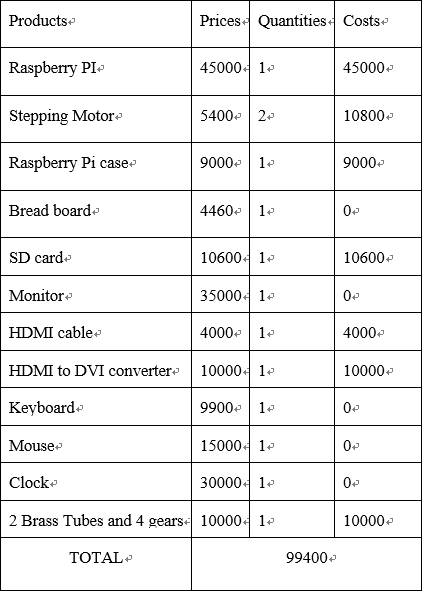
\includegraphics[width=0.45\textwidth]{Figure5.png}
			\caption{Caption2}
			\label{fig2}
			\end{figure} 
		\subsubsection{0.3.3.4. Using any commercial cloud platform}
			\begin{enumerate}
			\item Android developing \\
			- Windows: 10 \\
			- Android Studio: 2.3.1 \\
			\item Server developing \\
			- Ubuntu: 14.04.3 LTS \\
			- Java: 1.7.0.121 \\
			- Python: 3.4.3 \\
			\item Raspberry Pi developing \\
			- Raspbian: 4.4 \\
			\end{enumerate} 
	\subsubsection{0.3.3.5. Which member is responsible for what?}
		\begin{enumerate}
		\item Amazon's EC2 \\
		\item Software in use \\ \\
		a.‘Life 360’ Family location Tracking \\
			\begin{figure}[h]
			\centering
			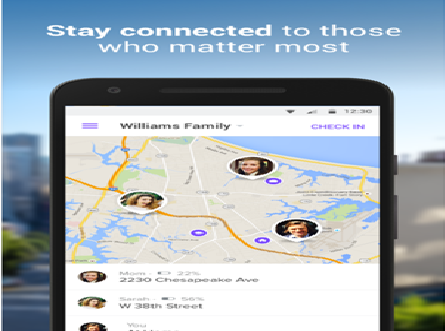
\includegraphics[width=0.45\textwidth]{Figure1.png}
			\caption{Caption3}
			\label{fig3}
			\end{figure} \\
		It is an application that shows each family member’s location for other family users. It can identify the family location at the same time. \\ \\ \\\\\\
		
		 b.	Traccar API \\ \\
		 Traccar API is tracing the location and showing the coordinates. This Traccar API is provided for Open Source.\\ \\
		 
		 c.	Google Maps API \\ \\
		 Google Maps API provides a map that User wants to see a coordinates that people is located. \\ \\
		 
		 d. RPI.GPIO modules \\ \\
		 We use a RPI.GPIO modules for controlling the GPIO. RPI.GPIO modules can control the stepping motor that is used for our Whereabouts clock. \\ \\
		 
		 e.	Github  \\ \\
	  Github was the environment we had to be used to. It is a free cooperation development tool for software development. It is a hosting service based on git, gathering all kinds of source. \\ \\
		 - Pull request \\
		 - Schedule management, report bug. \\
		 - Co-working is possible for other team as well as my team.\\ \\
		
		f.	Sublime text \\ \\
		Recently a lot of people use Sublime text. Sublime Text is a sophisticated text editor for code, markup and prose. Also, people can add any kind of functions other people made. Here are the features of Sublime Text include the following:  \\ \\
		
		 - Goto Anything \\
		 - Command Palette \\
		 - Split Editing \\
		 - Customize Anything \\
		 - Multiple Selections \\
		 - Distraction Free Mode \\
			\begin{figure}[h]
				\centering
				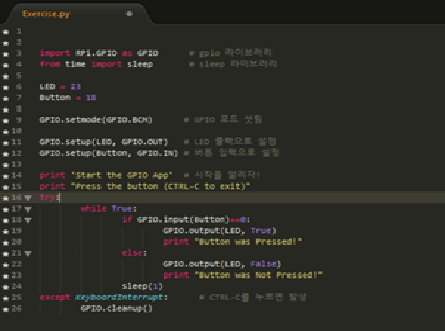
\includegraphics[width=0.5\textwidth]{Figure2.png}
				\caption{Caption4}
				\label{fig4}
			\end{figure} \\ \\\\

       g.	Android Studio  \\ \\		 

       Android Studio is the official integrated development environment (IDE) for the Android platform.Based on JetBrains' IntelliJ IDEA software, Android Studio is designed specifically for Android development. \\ \\
       \begin{figure}[h]
				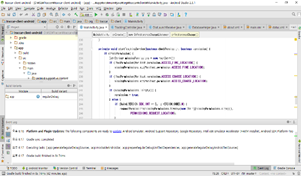
\includegraphics[width=0.5\textwidth]{Figure3.png}
				\caption{Caption5}
				\label{fig5}
		\end{figure} \\\\
		\item Task distribution (We will provide detail about this table later at the next design phase) \\
		 \end{enumerate}
		 
\section{SPECIFICATIONS}
	\subsection{Modeling for Specifications}
	 	\begin{figure}[h]
				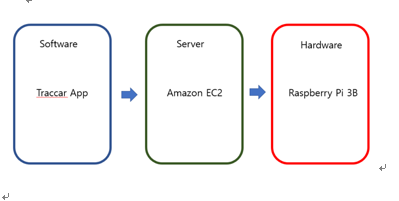
\includegraphics[width=0.5\textwidth]{Figure6.png}
				\caption{Caption6}
				\label{fig6}
		\end{figure}
		After receiving User’s location in Traccar App, we provide this information to Amazon EC2. Then Amazon EC2 compares the user’s location and default place location coordinates. And then the result is provided to Raspberry Pi 3. \\ 
		 
		 \begin{enumerate}
		 
		 \item find out User’s location in Traccar App.
		 \item deliver User’s location to Amazon EC2. 
		 \item Compare the user’s location and default place location 
		 \item If the result is changed, Amazon EC2 deliver the result to Raspberry Pi. 
		 \item Raspberry Pi is controlling the stepping motor. 
		 \item Whereabouts clock is turning according to User’s location. 
 		\end{enumerate}
 	\subsection{Specification Application}
 		\subsubsection{0.4.2.1. Sign in and login}
 		- It is the first page of the Whereabouts application. After entering the member ID, password, name, name, position of the household, and serial number of the clock. Once the sign-in is signed, the login window appears. We should always place a check box for keeping the log in.\\
 		\subsubsection{0.4.2.2. Permitting to give users GPS data}
 		- Get permission to receive GPS data from your mobile device directly after you log in. If rejected, close down the app with a message stating that the application cannot proceed.\\
 		\subsubsection{0.4.2.3. Setting the default location information ex) school – GPS data }
 		- Provide a map API to set the default location such as school, workplace, and home. Also, they enter the radius to be recognized as the same place. Enter this location name, latitude, and longitude to send to the server.\\
 		\subsubsection{0.4.2.4. Settings and On/Off for location information}
 		- Display the screen where you can set the server address, port number, location transfer time frequency, and location provider as shown in the following figure. Users can also control On/Off on this screen. \\
 		\begin{figure}[h]
				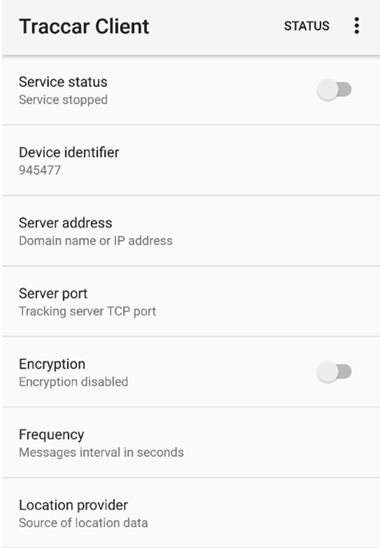
\includegraphics[width=0.5\textwidth]{Figure7.png}
				\caption{Caption7}
				\label{fig7}
		\end{figure}
 		\subsubsection{0.4.2.5. Transmitting GPS Information to Server}
 		- Sends a location to the server at regular intervals to accommodate the existing server address and frequency. Applications are implemented to operate in the background even if they are not opened on the screen of the mobile device.\\
 		\subsubsection{0.4.2.6. Members of Family List}
 		- Display the list of users whose names match with serial number of the clock and the corresponding user name of the clock that the member entered. Here, you can write and share a short state message within 30 characters. \\
 	\subsection{Specification Server}
 		\subsubsection{0.4.3.1. Service start}
 		- Access the Amazon EC2 Ubuntu environment using Putty. Then, launch the service by running startDaemon.sh in the /opt/traccar/bin folder \\
 		\subsubsection{0.4.3.2. Sign - up and login processing}
 		- When registering a user's membership, check whether the ID and the position of family are overlapped or not, and if a valid serial number are entered. Also, verify the identity of the ID and password when signing. \\
 		\subsubsection{0.4.3.3. Receiving GPS data and storing}
 		- Input the ID, latitude, longitude, and serial number from the mobile application and store them on the positions table in the MySQL. \\
 		\subsubsection{0.4.3.4. User position determination}
 		- Store the default location from the mobile application on the locations table. After comparing it to the location of the current user's latitude, longitude determine the user’s place. Send data to the clock if the user changes the location of the user.\\
 		\subsubsection{0.4.3.5. Transmitting the data to the clock}
 		- Find the clock serial number of a family member whose location changes occurred. Then use a protocol which is set beforehand to notify the change of location to the Raspberry Pi in the corresponding clock \\
 	\subsection{Specification Server}
 		\subsubsection{0.4.4.1. Receiving data from Amazon EC2 server }
 		- We receive user’s location from Amazon EC2 server. Originally, User location is received from Traccar App.  Traccar App gives a Real User’s location to Amazon EC2 server. And Amazon EC2 compares Real User location and default place location information. If the information compared to using Amazon EC2 is changed, Raspberry Pi 3 can notice the change.
 		\begin{figure}[h]
				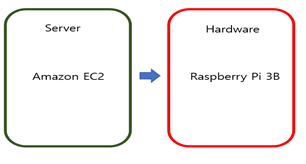
\includegraphics[width=0.5\textwidth]{Figure8.png}
				\caption{Caption8}
				\label{fig8}
		\end{figure}
 		\subsubsection{0.4.4.2. Handling input data}
 		- If Raspberry Pi 3 notice the change, Raspberry Pi 3 can control the GPIO modules. We use a RPI.GPIO modules using Python programming language. RPI.GPIO module controls the GPIO that uses to control the stepping motor. \\
 		\begin{figure}[h]
				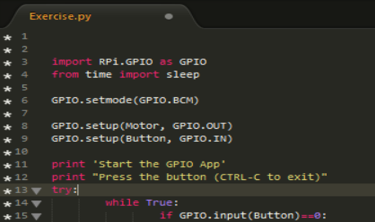
\includegraphics[width=0.5\textwidth]{Figure9.png}
				\caption{Caption9}
				\label{fig9}
		\end{figure}
		\subsubsection{0.4.4.3. Moving clock hands}
		- If the GPIO module controls the stepping motor, stepping motor turns to destination that indicates User Real location. Concretely, Stepping Motor turns a gear that connects from Brass Tubes. The gear makes clock spin to turn heading for the destination. \\
		\begin{figure}[h]
				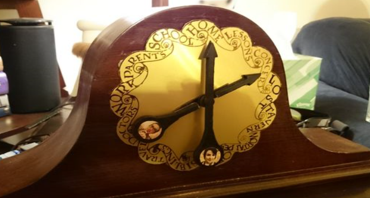
\includegraphics[width=0.5\textwidth]{Figure10.png}
				\caption{Caption10}
				\label{fig10}
		\end{figure}
		
\section{Architecture}
	\subsection{Overall Architecture}
		\begin{figure}[h]
				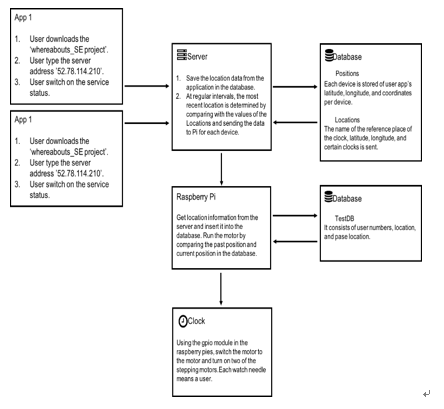
\includegraphics[width=0.5\textwidth]{Figure11.png}
				\caption{Caption11}
				\label{fig11}
		\end{figure} 
	
		\subsubsection{0.5.1.1. App 1, App 2}
		- User downloads the ‘whereabouts SE project’ \\
		- User type the server address ’52.78.114.210’ \\
		- User switches on the service status. \\
		
		\subsubsection{0.5.1.2. Server}
		- Save the location data from the application in the database.\\
- At regular intervals, the most recent location is determined by comparing with the values of the Locations and sending the data Pi for each device.\\
		\subsubsection{0.5.1.3. Server Database}
		- Positions DB: Each device is stored of user app’s latitude, longitude, and coordinates per device.\\
- Locations DB: the name of the reference place of the clock, latitude, longitude, and certain clocks is sent.\\
		\subsubsection{0.5.1.4. Raspberry Pi}
		-  Get location information from the server and insert it into the database. Run the motor by comparing the past location and current position in the database \\
		\subsubsection{0.5.1.5. Raspberry Pi Database}
		- TestDB: It consists of user numbers, location and past location.\\
	\subsection{Directory architecture}
		\begin{figure}[h]
				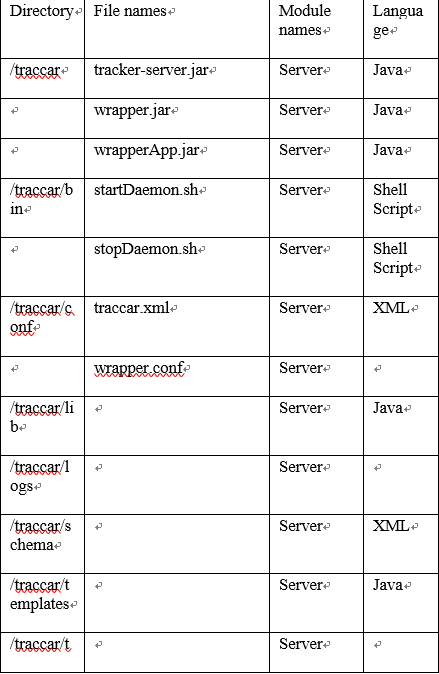
\includegraphics[width=0.5\textwidth]{Figure12.png}
				\caption{Caption12}
				\label{fig12}
		\end{figure} 
		\begin{figure}
				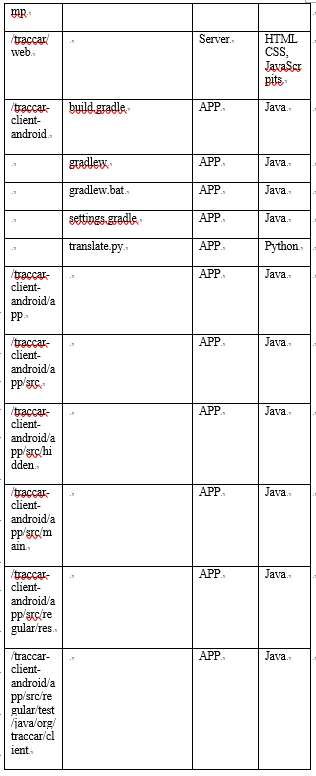
\includegraphics[width=0.5\textwidth]{Figure13.png}
				\caption{Caption13}
				\label{fig13}
		\end{figure} 
		\begin{figure}
				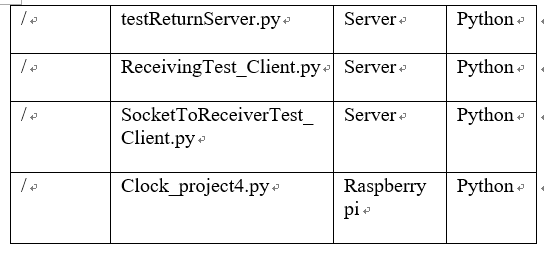
\includegraphics[width=0.5\textwidth]{Figure14.png}
				\caption{Caption14}
				\label{fig14}
		\end{figure} 
	
	
	
	\subsection{Software Component}
		\subsubsection{0.5.3.1. Software Component 1: Application}
		\begin{enumerate}
		\item Purpose \\
		- Application is useful for delivering user’s location in Server. Our Whereabout clock catches user’s location using GPS. \\
		\item Functionality \\
		- Application delivers Id, protocol, deviceid, servertime timestamp, fixtime, valid, latitude, longitude, altitude, speed, course, address, attributes, accuracy, network attributes in Server Database ‘Position’ Table.\\
		\item Location of Source Code \\
		- /traccar-client-android \\
		\item Class Components \\\\
		4-1. Bulid.gradle \\ \\
		- CompileSdkVersion = 25 \\
		- TargetSdkVersion 25 \\
		- MinSdkVerison = 3 \\
			\begin{figure}[h]
				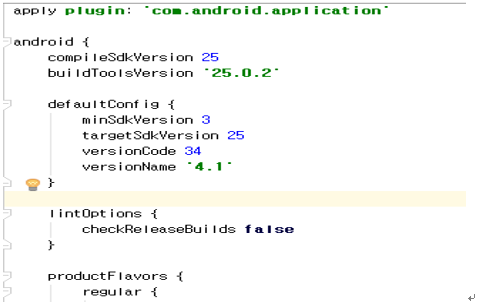
\includegraphics[width=0.5\textwidth]{Figure15.png}
				\caption{Caption15}
				\label{fig15}
			\end{figure}  \\\\\\\\\\\\\\\\\\
			
			
		4-2. PositionProvider \\
		- ‘locationManager = (LocationManager) context.getSystemService (Context.Location. \\SERVICE)’ is a source code that get actually user’s location using Applicatoin \\
		
		\begin{figure}[h]
				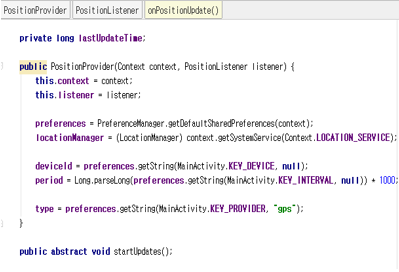
\includegraphics[width=0.5\textwidth]{Figure16.png}
				\caption{Caption16}
				\label{fig16}
		\end{figure}
		
		\item Where it is taken for? \\
		= https://github.com/tananev/traccar-client-android.git \\
		\begin{figure}
				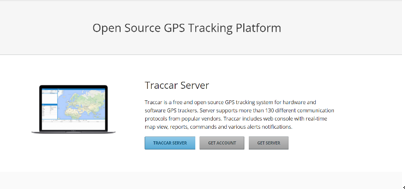
\includegraphics[width=0.5\textwidth]{Figure17.png}
				\caption{Caption17}
				\label{fig17}
		\end{figure}
		
		\item How/Why you used it? \\
		- Users can use this app to display location on the clock. Specifically, Users turns on the App and register Server IP address in this App. This app sends user’s latitude and longitude to the server. So, the server will then receive the latitude and longitude of the user \\
		\end{enumerate}
	\subsubsection{0.5.3.2. Software Component 2: Server}
		\begin{enumerate}
			\item Purpose\\
			- The server receives the user’s location through the app. Then the server stores the user’s location in its database. It processes the user’s location and data on the server itself. This will allow to send a user data and user location to Raspberry pi 3.\\
			\item Functionality \\
			- Server will do many things. The first thing is to store the user’s location in the database through the app. And Server picks up the user’s location from the database and handles the value. Processed values will be sent to the raspberry pi 3 Server. \\
			\item Location of Source Code \\
			- /traccer \\
			\item Class Components \\\\
			4-1. startDaemon.sh \\
			- This is portion that the server operates. This file allows the user to store the location of the users that Android delivers to the server. \\
			\begin{figure}[h]
				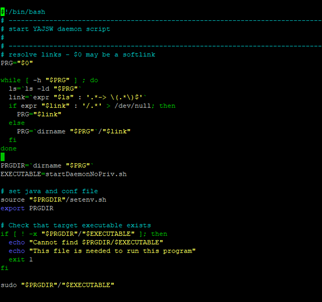
\includegraphics[width=0.5\textwidth]{Figure18.png}
				\caption{Caption18}
				\label{fig18}
			\end{figure}
			\\\\\\\\\\\\\
			4.2. testReturnServer.py \\
			- This is the portion of getting the user’s location that is recalled from the Potion database table. The User’s location is sent to raspberry pi after processing user’s location in an easy manner. \\
			\begin{figure}[h]
				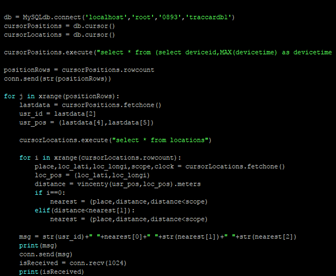
\includegraphics[width=0.5\textwidth]{Figure19.png}
				\caption{Caption19}
				\label{fig19}
			\end{figure}
			\\\\\\\\\\\\\
			4.3. ReceivingTest.Client.py \\
			- When the ReceivingTest.Client.py runs, it sends the user’s location to Raspberry pi database. The user’s pin number and the user’s location are sent to Raspberry pi database. \\
			\begin{figure}[h]
				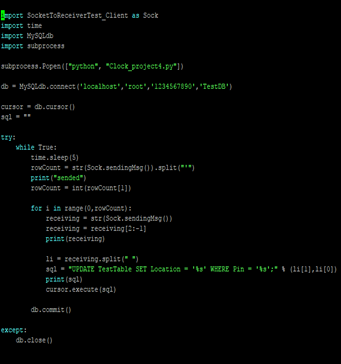
\includegraphics[width=0.5\textwidth]{Figure20.png}
				\caption{Caption20}
				\label{fig20}
			\end{figure}
			\\\\\\\\\
			4.4. SocketToReceiverTest.Client.py \\
			- Server sends a user’s pin number and user’s location through a socket. \\
			\begin{figure}[h]
				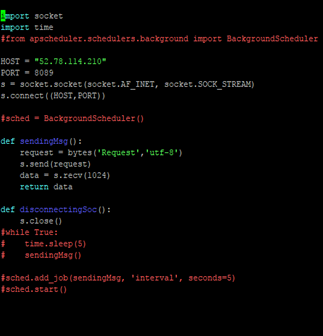
\includegraphics[width=0.5\textwidth]{Figure21.png}
				\caption{Caption21}
				\label{fig21}
			\end{figure}
			\\\\\\\\\\\\\\\\\\\\\\\
			\item Where it is taken for?  \\
			\begin{figure}[h]
				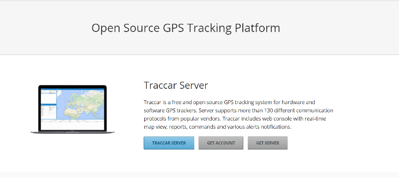
\includegraphics[width=0.5\textwidth]{Figure22.png}
				\caption{Caption22}
				\label{fig22}
			\end{figure}
			\item How/Why you used it? \\
			- The server obtains the user’s location from the app. Bring the user’s location in the database and process the data easily to send to the raspberry pi 3. Then pass the data to the clock by passing the user onto the raspberry pi 3. \\
	\subsubsection{0.5.3.3. Software Component 3: Raspberry pi}
			1. Purpose \\
			- Raspberry pi 3 is essential for rotating our clock. The raspberry pi 3 gives electrical signals to the stepping motor. And the stepping motor which receives electrical signals turns to the direction that describes the location of the user. \\\\
			2. Functionality \\
			- The raspberry pi 3 calls the user’s location from the server. The user’s location is stored in the raspberry pi ‘TestDB’ database. The raspberry pi 3 steer the stepping motor according to the direction of the specified direction. Raspberry pi 3 uses the ‘RPi.GPIO’ modules. It is useful for sending signal to the stepping motor. ‘RPi.GPIO’ module is used in Python. \\\\
			3. Location of Source Code \\
			- /Clock.project4.py \\\\
			4. Class Components \\\\
			4-1. Clock.proejct4.py -1 \\\\
			- This Source code is a part that accesses the ‘TestDB’ database and receives the user’s location. \\
- ‘sendSignal()’ method is sending electrical signal to the GPIO in Raspberry pi 3. \\
- ‘numberTest()’ method is identifying who the user is.\\
- ‘test1()’ method is identifying where the user is located \\
			\begin{figure}[h]
				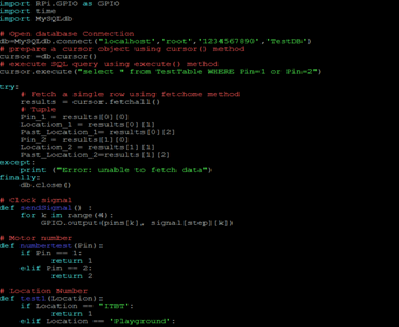
\includegraphics[width=0.45\textwidth]{Figure23.png}
				\caption{Caption23}
				\label{fig23}
			\end{figure}
			\\\\\\\\\\\\\\\\\\\\\\\\\
4-2. Clock.proejct4.py -2 \\\\
-‘test2()’ method is identifying where the user is located
- ‘Angletest1()’ method compares the user’s past location with the current position and specifies the angle at which the clock is rotated. \\
			\begin{figure}[h]
				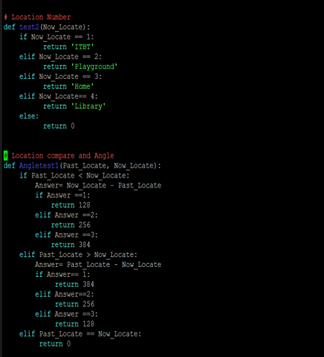
\includegraphics[width=0.45\textwidth]{Figure24.png}
				\caption{Caption24}
				\label{fig24}
			\end{figure}
			\\\\\\\
			4-3. Clock.proejct4.py -3 \\\\
			- ‘main()’ method is actually part of the action. It obtains the location of the user from the database. It processes the signals to be sent to the motor thorough the process of testing the user and testing the user’s location. \\
			\begin{figure}[h]
				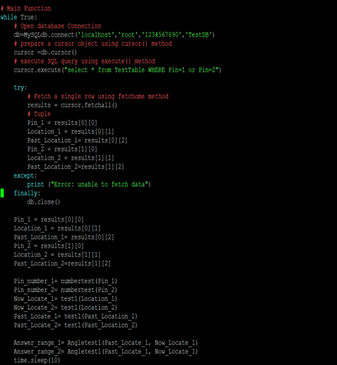
\includegraphics[width=0.47\textwidth]{Figure25.png}
				\caption{Caption25}
				\label{fig25}
			\end{figure}
			\\\\\\
			4-4. Clock.proejct4.py -4 \\\\
			- If the user current location and past location differ, this part moves. And if the pin number is one, this part moves. Raspberry pi 3 sends electrical signals to pin 12, 14, 20, 21 At this point, it is moved by a predetermined angle.\\
			\begin{figure}[h]
				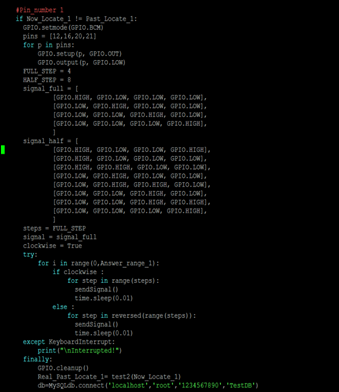
\includegraphics[width=0.47\textwidth]{Figure26.png}
				\caption{Caption26}
				\label{fig26}
			\end{figure}
			\\\\\\\\\\\\\\\\
			4-5. Clock.proejct4.py -5 \\\\
			- If the user current location and past location differ, this part moves. And if the pin number is two, this part moves. Raspberry pi 3 sends electrical signals to pin 6, 13, 19, 26 At this point, it is moved by a predetermined angle. \\
- Finally, after turning the motor, save the current user’s location in the ‘Past.Location’ column. \\
			\begin{figure} [h]
				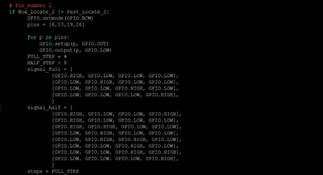
\includegraphics[width=0.47\textwidth]{Figure27.png}
				\caption{Caption27}
				\label{fig27}
			\end{figure}
		\\\\
		5. Where it is taken for? \\ \\
- Blog Address: https://codefooo.gitbooks.\\io/raspberry-experiments/content. \\
- We refer to this blog to turn around the stepping motor. \\
			\begin{figure}[h]
				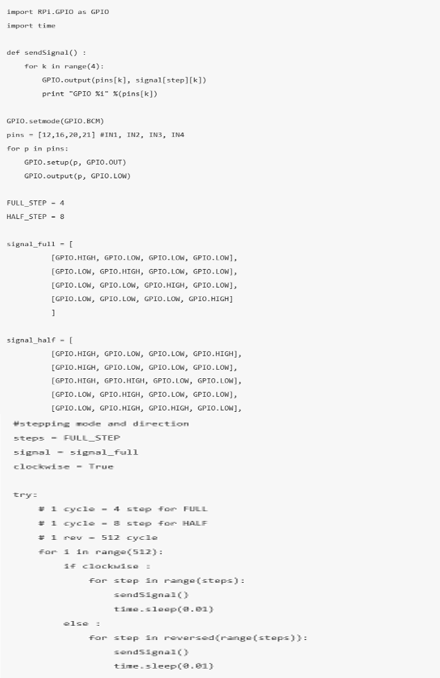
\includegraphics[width=0.5\textwidth]{Figure28.png}
				\caption{Caption28}
				\label{fig28}
			\end{figure}
		\\\\
		6. How/Why you used it? \\\\
		- Raspberry pi 3 is currently used in many places. Raspberry pi 3 is a small computer that you use to turn a stepping motor. You can create a program by using a python and sending electrical signals to the GPIO. We used RPI.GPIO modules for sending signals to the GPIO. We can rotate the two stepping motors depending on the location of the user.\\	
		\end{enumerate}
		
		
\section{Use Cases}		
	\subsection{Main Use Cases}
		\subsubsection{0.6.1.1. Download Our Application}
		- User downloads our Whereabouts-SE Project APP in google store. \\
		\begin{figure}[h]
				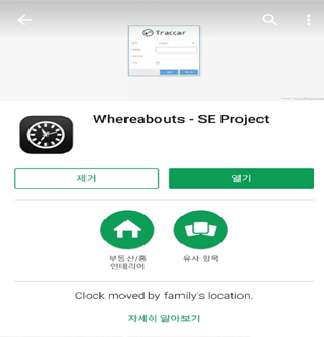
\includegraphics[width=0.5\textwidth]{Figure29.png}
				\caption{Caption29}
				\label{fig29}
			\end{figure}
		\\\\
		\subsubsection{0.6.1.2. Permit to use GPS}
		- Second, if User installs Whereabouts – SE Project Application, User permits to the use GPS in the App. This function allows App to use User’s GPS data.\\
		\subsubsection{0.6.1.3. Put the Amazon EC2 Server Address}
		- User puts the Amazon EC2 Server Address in the Whereabouts – SE Project App. So, User’s Location is sent to Server.\\
		\begin{figure}[h]
				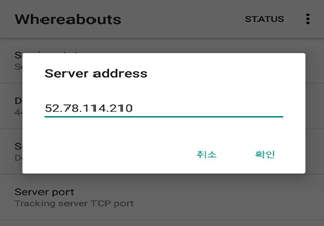
\includegraphics[width=0.5\textwidth]{Figure30.png}
				\caption{Caption30}
				\label{fig30}
		\end{figure}
		\subsubsection{0.6.1.4. Set the Frequency}
		- User set the Frequency that request to the Amazon EC2 Server. \\
		\begin{figure}[h]
				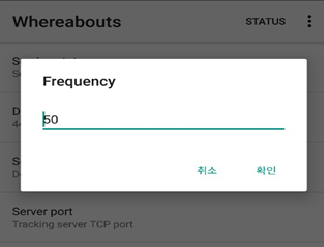
\includegraphics[width=0.5\textwidth]{Figure31.png}
				\caption{Caption31}
				\label{fig31}
		\end{figure}
		\subsubsection{0.6.1.5. Select location provider between GPS mode and Network mode}
		- User selects location provider between GPS mode and Network mode.\\
		\begin{figure}[h]
				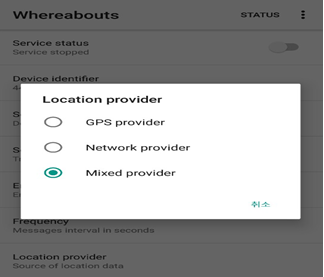
\includegraphics[width=0.5\textwidth]{Figure32.png}
				\caption{Caption32}
				\label{fig32}
		\end{figure}
		\subsubsection{0.6.1.6. Service Start}
		- After User finished app setting, User can use the Clock Service. User’s location is sent to Server. And Server knows User’s real location. So, Server sends a user’s location to Raspberry pi. \\
		\subsubsection{0.6.1.7. Connect the Clock power}
		- User should connect the Raspberry pi power in the socket. So, Clock can be rotated thorough User’s real location.  \\
			 
\end{document}